\documentclass[11pt]{article}
%\usepackage{acl2015}
%\usepackage{times}
\usepackage{latexsym}
\bibliographystyle{ieeetr}
\usepackage{amsmath}
\usepackage{multirow}
\usepackage{url}
\usepackage{booktabs}
\usepackage{graphicx}					% to include graphics
\graphicspath{{pics/}}						% folder for graphics


\begin{document}


\title{Semi-Supervised Learning for Semantic Textual Similarity}

\author{Tim Powell}

\date{}
\maketitle

\begin{abstract}
Semantic textual similarity tasks involve rating the degree of similarity between two pieces of text, either sentences or passages. I experiment with a variety of approaches for predicting similarity, focusing on a task in which the test data presented is of a different domain from the training data. No improvement is detected by using semi-supervised domain adaptation approaches, while stronger correlations are found by dropping some of the training data, as well as relying on a sentence overlap measure without training. \
\end{abstract}


\section{Introduction}
 
Previous approaches to domain adaptation for semantic textual similarity have made use of feature augmentation strategies \cite{heilman2013ets} \cite{severyn2013ikernels} and by transferring only a subset of the source data for predicting on the target data \cite{arora2015dcu}. Given the requirements set out by the competition format in which these experiments take place, no data outside the permitted training corpora is used for domain adaptation. My experiment sets out to investigate whether performing semi-supervised learning can provide superior results, through the use of unlabelled target-domain data.  I follow only a subset of the feature representation steps taken in \cite{arora2015dcu}. The syntactic features, sentence embeddings and cosine similarities between sentence pairs seem to provide sufficient information to approximate the authors' results (which relies on wider range of features). The effectiveness of semi-supervised methods is inconclusive, as results on out-of-domain test data are not improved following two approaches which involve unlabelled target-domain data. One approach, self-training, creates target-domain data by first training on source-domain data, and making predictions on unlabelled data, which is then concatenated with the labelled training data. On the other hand, tri-training performs a similar labelling of target data through the predictions of three predictors, fitted on labelled source-data. While these approaches fail to improve scores on the test data, a simple domain adaptation technique, whereby training instances are filtered by similarity to the test data, presents mixed results in both previous experiments and my own.\\

\section{Data and Resources}
Semeval's Semantic Textual Similarity task is a yearly competition where participants submit their approach to measuring the similarity of two sentences. New test data is provided every year, and competitors train their models on the previous years' corpora. The English test data for 2015 covers 5 domains: answers from stackexchange.com, sentences from the DEFT annotated committed belief dataset, news headlines, answers provided by students using a tutorial dialogue system, newswire headlines and image descriptions\cite{agirrea2015semeval}. The first two domains are not provided in any of the previous years' competitions. My domain adaptation approach relies on additional data from stackexchange.com. I have scraped over 8000 sentences from answers in the same topics used for the task's test data (cognitive science, academia, astronomy, etc) Following \cite{arora2015dcu}, I train my first model on the train and test data from 2012-1014.  \\

I am using Gensim's Word2Vec package and have trained a model on the wikipedia text8 corpus combined with my training data \cite{rehurek_lrec}. I am using Sci-kit Learn's regression models for training, self-training and tri-training (Decisions Tree, Ridge Regression, and SVR) \cite{scikit-learn}\\

\section{Methodology}
\subsection{Preprocessing}
My approach requires two levels of pre-processing. Training and test data are stemmed using the Porter stemmer, and stop words are removed, using NLTK's libraries \cite{BirdKleinLoper09}. These extra steps are taken when creating features that correspond to basic and weighted similarity scores between sentence pairs (as stemming prevents dissimilar scores due to inflections and derivations and stop words may return artificially high similarity scores). I am only applying my first level of preprocessing for features corresponding to sentence embedding similarity scores, and syntactic features. This involves filtering out non-alphanumeric characters, converting to lowercase and tokenizing.  \\

\subsection{Feature Design}
\subsubsection{Cosine similarity}
My first two features correspond to the cosine similarity between two variations of the sentence pairs' vector representations. Both vectors are the length of the vocabulary size and comprise of zeros except for indices representing words occurring in the sentence. At these indices, a one is placed when calculating the basic cosine similarity. For the weighted cosine similarity, the vectors consist of zeros and Inverse Collection Frequency scores at indices of occurring words.  ICF scores are calculated by taking the log of the corpus' total word count over the frequency of word $i$ over the corpus, scaled by the log of the total word count. These scores are calculated only over the training corpus.
I measure the similarity between sentence pairs in vector space by calculating the cosine of the angle between the vectors $x$ and $y$, corresponding to sentence 1 and sentence 2:\\

$cos(\pmb x, \pmb y) = \frac {\pmb x \cdot \pmb y}{||\pmb x|| \cdot ||\pmb y||}$



\subsubsection{Sentence Word2vec}
An additional feature used in \cite{arora2015dcu} involves 'sentence embeddings' by calculating the cosine similarity between the averages of a sentence pair's word embeddings.  A neural network with one hidden layer is trained on the training corpus to produce vector representations for each word. The training of the model works with the assumptions of distributional semantics, such that words which appear in similar contexts will return similar vectors. The vectors representing word embeddings are, however, not what the neural network outputs. Using skip-gram as a training algorithm, the model takes as input one word (as a one-hot encoding vector) in a context window of size 5 and minimizes the error between the one-hot encoding vector of every other word in the context and the output value.  Hierarchical softmax is used for efficiency to represent the output values as normalized probabilities and the weights are updated by stochastic gradient descent. The weights are initialized randomly and once the training has converged, the weights from the input layer to the hidden layer are retrieved as a vector for a word embedding \cite{mikolov2013efficient}. I have set this vector to be of dimension size 100.  At testing, words from a sentence pair that are not in the model are ignored when calculating centroids for cosine comparison. \\

\subsubsection{POS Tag}
Using NLTK's Part-of-Speech tagger, (a perceptron tagger pre trained on English data) I extract two sets of syntactic features related to four coarse-grained POS tags (NN, VB, RB, JJ). The first set involves calculating a cosine similarity of the sentence embeddings for each POS tag, as outlined above, using the mean of all terms tagged as POS tag $i$. The second set produces a simple count of the terms in both sentences that are lexical matches and share the same POS tag (a count is kept for each POS tag).  \\
\subsection{Baseline}
My baseline approach calculates a simple overlap score between sentence pairs, without training. Sentences are tokenized, non-alphanumeric characters are removed, as are stop words. I take the intersection of both pre-processed sentences over the length of either sentence. The mean of these two values is scaled by five in order to conform to the task's scoring format. \\
\subsection{Domain Adaptation}

\subsubsection{Data selection}
As some of the test data for this task is from a domain not found in any of the training data, one of the domain adaptation methods employed by \cite{arora2015dcu} is to train a model on parts of the training corpus that are similar to the test data. I build a focused subcorpus by collecting five sentence pairs from the training data that have the highest cosine similarity to every out-of-domain test instance. No additional unlabelled data is required in this approach, as I'm simply dropping source domain data that has a higher divergence from my target domain. \\
\subsubsection{Self-training}
Self-training is an approach for domain adaptation which makes use of unlabelled data taken from the target domain, to compensate for a bias resulting from training a predictor on the labelled source domain.  Once a predictor $C$ is trained on labelled data $L$, the predictions made on unlabelled data $U$ are used as labelled data on which the same predictor is trained again. Only a subset of the unlabelled data is used for labelling and re-training per iteration. In this experiment, self-training is performed over a concatenation of the labelled data and 10 newly labelled sentence pairs, retrieved from a similar domain as the 'answers-forum' test data. \\
\begin{table*}[]
\centering
\caption{Results}
\label{results}
\begin{tabular}{|l|l|l|l|l|l|}
\hline
Test set         & Baseline & BaselineTP & Basic Train & Foc. Corp & F.C., Arora \\ \hline
Images           & 0.6039   & 0.8266     & 0.8262      & -              & 0.8434                       \\ \hline
Headlines        & 0.5312   & 0.7771     & 0.7595      & -              & 0.8181                       \\ \hline
Belief           & 0.6517   & 0.719      & 0.706       & 0.7142         & 0.6977                       \\ \hline
Ans-students & 0.6647   & 0.707      & 0.6711      & 0.6881         & 0.6108                       \\ \hline
Ans-forum    & 0.4453   & 0.7308     & 0.6376      & 0.6359         & 0.653                        \\ \hline
\end{tabular}
\end{table*}
A grid search performed over parameters of a Support Vector Regression model returns a C value of 10 and a gamma value of 0.01 as optimal parameters for training on the labelled data. \\
\subsubsection{Tri-training}
In tri-training, three predictors are trained on the labelled data, and two of these predictors are used for labelling a subset of the unlabelled data. If there is agreement in these predictions, the newly labelled data points are used for retraining of the third predictor. This process is repeated over several iterations, cycling through three arrangements of the models for prediction and retraining, in order to return one predictor. For this experiment, I am performing 30 iterations and returning a Support Vector Regression predictor, informed by the predictions of Kernel Ridge Regression and Decision Tree regression models -- which at each iteration are themselves informed by predictions of the other two predictors.) At every iteration, every model is retrained on a subset of 50 data points of the unlabelled data if the two predictions of the other models fall within 0.2 in similarity score of each other. In which case the mean of the two scores is used for retraining. \\

The decision tree's maximum depth is set to 5 and the Kernel Ridge Regressor's alpha and gamma values are set to 0.01, following parameter optimization performed over different values.\\

\section{Results}
The results table \ref{results} shows Pearson correlation scores for different approaches to semantic textual similarity, with a score given at every domain (between system output and gold standards). The first column represents the Pearson correlation scores for SemEval's 2015 STS task's baseline, which tokenizes sentence pairs and returns the cosine similarity. My baseline, explained above, produces results listed in the second column. The third column's Pearson scores are produced without any domain adaptation method, simply by fitting an SVR model to all the training data. A model is also fitted on a subset of the training data, as outlined previously, and listed in the fourth column (Focused Corpus). The authors use a similar domain adaptation approach for one of their three submitted runs, which is listed in the final column. Figures \ref{fig:selftraining} and \ref{fig:tritraining} show Pearson correlation scores between the output of the model and gold standards, for self-training and tri-training, respectively. \\
\begin{figure}[h]
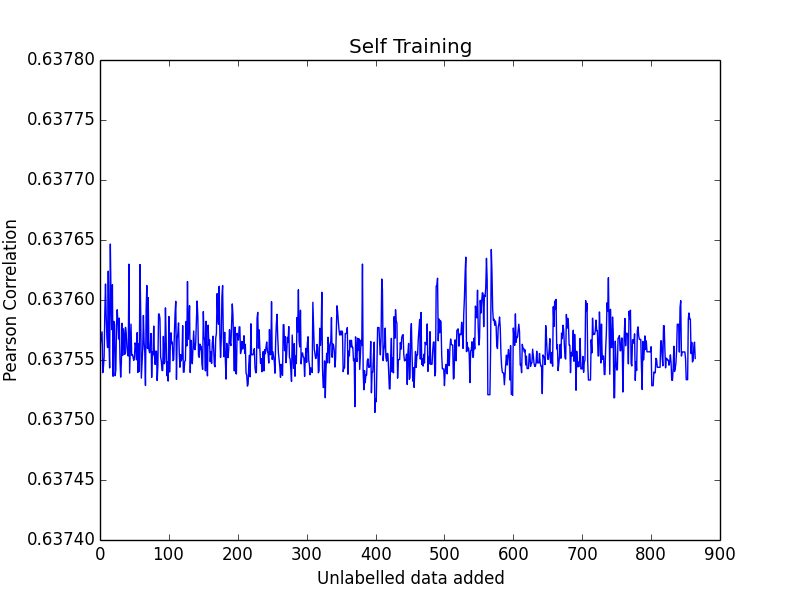
\includegraphics[width=9cm]{selftraining}
\caption{Self Training}
\label{fig:selftraining}
\end{figure}

\begin{figure}[h]
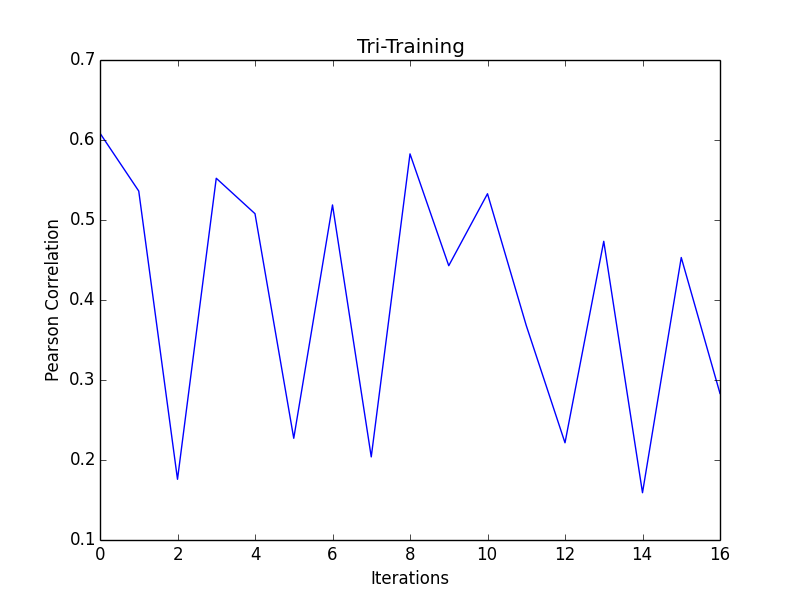
\includegraphics[width=9cm]{tritraining}
\caption{Tri Training}
\label{fig:tritraining}
\end{figure}


\section{Discussion}
Most surprising of all results is the strong performance of what had been set up as a simple baseline. This approach which calculates the overlap between sentences, outperforms an SVR model, trained on a collection of syntactic and semantic features, either from all training data or a focused subset. Results in \cite{arora2015dcu} also fail to beat this overlap measure in cases where the domain of the test data is not found in the training data (i.e., the last three rows). Despite the presumed simplicity of the measure, a heuristic which does not require any training can understandably outperform machine learning approaches if source domain bias is not adequately adapted for.\\

The results reveal that dropping data by cosine dissimilarity is a good domain adaptation technique, given the increase in performance between the basic training and the focused corpus training. Interestingly, my results for the 'Belief' and 'Answers-students' domains are better than those provided \cite{arora2015dcu}, suggesting that a more limited collection of features can capture similar information for textual similarity. Other than number of features employed, the authors research differs from mine in the algorithm used for training (M5P vs. SVR). \\

The failure of the self training approach to offer any increase in performance can be explained by several factors. It is possible that insufficient unlabelled data is used, as $L$ $>$ $U$. As noted in \cite{sogaard2013semi}, a handful of strategies could be used to improve performance of self-training: Retraining on newly labelled data only if a predictor's confidence of the label is high enough or using a smaller pooling of the unlabelled data.\\

The fluctuations in performance with tri-training are harder to explain. It is possible that inadequate model selection for tri-training has led to the use of low-performing predictors. However, two predictors would have to agree on their incorrect predictions for the unlabelled data to be used in re-training. Pooling size may also be a factor, as each model is retrained at a pooling size of 50. \\

\section{Further Research}
Further research should exploit the self-evident robustness of a measure that is impervious to source domain bias. Improved implementations of domain adaptation methods outlined above could be combined with a collection of similarity heuristics to achieve better results. Another improvement on the current experiment would involve a more thorough analysis of the unlabelled data, filtering out sentence pairs that are highly dissimilar based on simple cosine similarity. Avoiding any retraining on unlabelled data with a heavy class imbalance may prove to be a smarter approach.\\

\section{Conclusion}

In this paper, I have explored the use of semi-supervised domain adaptation methods to measure the semantic equivalence of sentence pairs. I have produced similar results to previous work with a more limited set of features, returning similar Pearson correlation scores between my system's predictions and human ratings of similarity on sentences from Semeval's Semantic Textual Similarity task, but have failed to show how self-training and tri-training may improve the robustness of a system. Future work could experiment with various strategies for improving on self-training, such as pooling size.  \\
\bibliographystyle{acm}
\bibliography{biblo}


\end{document}
